\documentclass{article}
\usepackage[dutch]{babel}
\usepackage{hyperref}
\usepackage{graphicx}


\title{Eindvergadering ML sessie 4}
\author{Team $\exists$uler \and
	\textit{Daan, Marie, Zeineb, Florian, Vincent, Jasper, Lasha, Younes}}
\date{Vrijdag \today}

\begin{document}
	
\maketitle

\section*{Reflectie}

In het begin van de sessie heeft iedereen zijn/haar machine learning techniek voorgesteld aan de rest van het team. We hebben in totaal 7 technieken besproken.

Uit deze technieken selecteerden we de beste 3, namelijk Neural Networks, Random Forests en Support Vector Machines. Deze 3 technieken hebben we vervolgens verdeeld onder elkaar voor verder onderzoek. Elke groep schreef een motivatietekst bij de aan hen toegekende techniek, en plaatste de tekst vervolgens in de OneDrive map \textit{Toepassing}:

\begin{itemize}
	\item Support Vector Machines: Jasper, Vincent en Younes (\textit{voorstel\_1\_TeamE.txt})
	\item Random Forest: Marie, Zeineb en Daan (\textit{voorstel\_2\_TeamE.txt})
	\item Neurale netwerken: Florian en Lasha (\textit{voorstel\_3\_TeamE.txt})
\end{itemize}

Wanneer we klaar waren met deze 3 technieken concreter uit te werken, hebben we verder gewerkt aan de oefeningen die nog open stonden in de KanBan.

\section*{Vooruitblik}

In de loop van volgende week zullen we de oefeningen verder afwerken. Oefeningen die we tijdens deze sessie hebben gemarkeerd als \textit{opnieuw}, zullen ook verbeterd moeten worden.

Vanaf het moment dat we onze extra machine learning techniek toegewezen krijgen, kunnen we concreet nadenken over mogelijke datasets die we kunnen gebruiken om deze techniek op toe te passen.

\begin{figure}
	\centering
	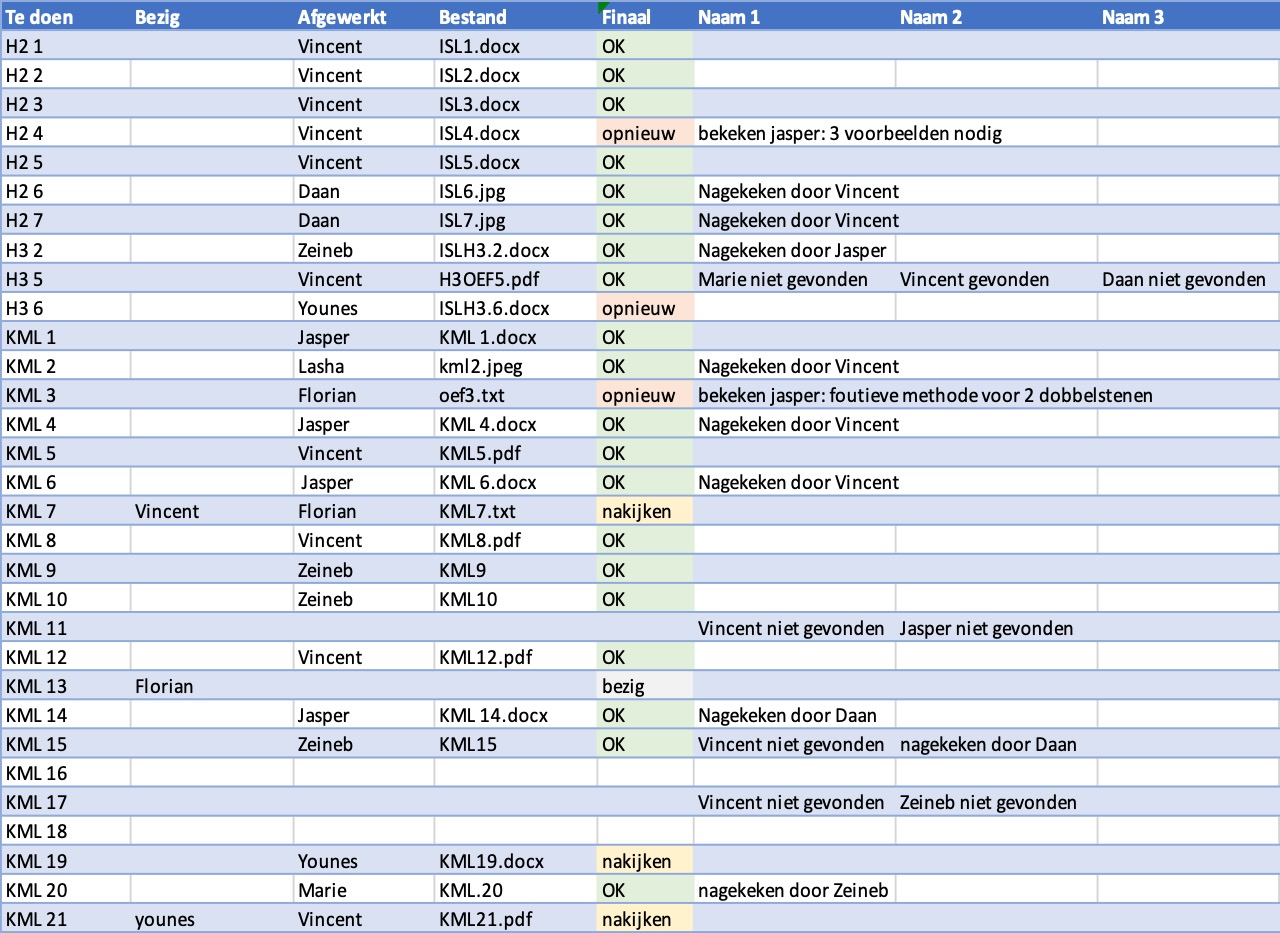
\includegraphics[width=12cm]{kanban}
	\caption{De status van het tabblad \textit{Oefeningen} in de KanBan aan het einde van sessie 4.}
	\label{fig:kanban}
\end{figure}

\end{document}